In the first sections of this chapter we outline the background, purpose and
objectives and the last section describes the scope of our research. Chapter 2
contains the theory needed for understanding the thesis, existing software and
some verification methods described in the standards. Methods is described in
Chapter 3 and the results in Chapter 4. In Chapter 5 and 6 we have a discussion
and some conclusions about the results.

%Background to the assignment. Why is it relevant?
\section{Background}
The last decade of the 20th century resulted in a dramatic growth of
technology(?). The rate is still increasing with up to 90\% of all innovations
being realized through electronics in the beginning of the 21st century (?), and
over 80 \% of all innovations in the automotive industry is in the electronics
and software area\cite{SAFE:interoperability}.
%% eventuellt dela upp paragrafen h�r d� det �r tv� olika ideer; en om att
%% teknologin utvecklas snabbt och mycket, och en som handlar om att just bilar
%% blir mer komplexa.
The software-based systems in motor vehicles have become more complex, and are
moving toward handling more critical functions (?). Vehicles have already begun
to communicate with each other \cite{VOLVO:convoys}, and it is soon expected
that roadside traffic management systems will also interact with the systems in
vehicles\cite{SURVEY:car_communications}.

While the systems become more complex the software must be fault-tolerant and
safe. Testing, validation and verification is a need and should follow all
product development phases, from start to finish. The problem is that testing
is %% introducerar "product development phases" utan f�rklaring. beh�vs den?
both time consuming and labour intensive, accounting for up to 50 \% of the
development cost\cite{QUICKCHECK:lightweight}. Unit tests adds additional
complexity to the code. It is very important to test and verify all steps of the
development.

The complexity issue is that in systems such as microprocessors the number of
possible failure modes is so large it is considered
infinite\cite{COURSEBOOK:safety-critical}. This makes it impossible exhaustively
test the system, and therefore, also make the detection of failures unreliable.

Quviq QuickCheck has the ability to automate this process, and allow the
developer to write properties instead of tests. These properties make it
possible for QuickCheck to create arbitrary input vectors that can be feed to
the code. Figure~\ref{IMG:phase_model} shows the different steps of the software
development process and the test and verification phases it has.

\begin{figure}[!ht]
  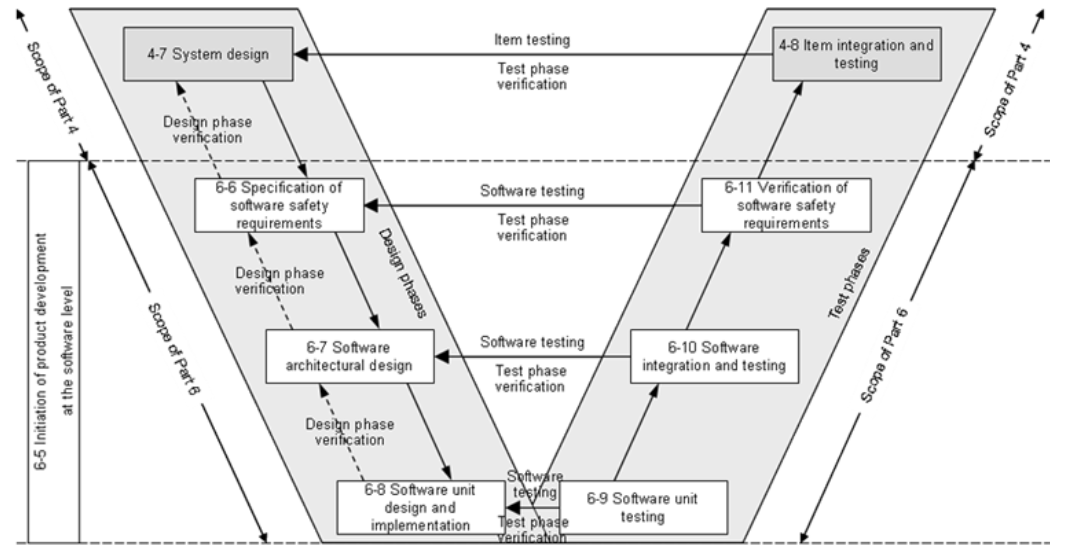
\includegraphics[keepaspectratio, width=\linewidth]{pictures/V}
  \label{IMG:phase_model}
  \caption{Phase model for software development}
\end{figure}

The first step is the system design. At this point the system specification is
written, and then the software specifications. When all specifications exists,
the next phase is to design the software architecture. The last part of the
design is software unit design and implementation. All phases must be a
verification of the former phase.

When the implementation is done, it is time for the test phases. These begins
with software unit testing which tests the software unit design phase. If the
tests verifies that the software unit design and implementation is correct, the
test phase moves on to the architectural design and then to verification of
software safety requirements.
The last test phase verifies that the system is
designed according to the specification. %It is important that the test phases
%test the specifications and not the
%implementation.

%Aim for the work. What should be accomplished?
\section{Purpose}
The purpose is to automate the testing process in an effective and good way.
To make it possible to raise the Automotive Safety Integration Level (ASIL), in
the software unit design and implementation phase and in the software %% n�mner
 %% ASIL utan att ha pratat om det tidigare.
architectural design phase, a check must be done to see if it exist a tool that
can be used in order to perform a semi formal verification of a module, and
then make this process generalized for modules in coexistence.\\ %% v�ldigt l�ng
 %% mening

The purpose is also to be able to decrease the number of needed unit tests in
the software unit design and implementation phase. Even further is the goal to
introduce semi formal verification of the software architectural design phase.
The functional safety concept will be most important in this phase.

%question formulation?
%The problem at hand, the assignment
\section{Objective}
The objective is to propose and motivate what should be done to be able to
achieve a semi formal verification. This should include a confidence interval
for how certain the verification is.

The objective is also to prove that it is possible to do semi formal
verification for an AUTOSAR module and its specification. This should be
generalized so its possible to test other specifications and modules at a later
moment. It should also not matter which configuration that is active, because
the specification should hold for all configurations.

%Limitations. What should be left out and why?
\section{Scope}
We will use AUTOSAR 4.0 revision 3 for our thesis work.
Since this version of AUTOSAR consists of around 80 specifications and other
auxiliary materials\cite{AUTOSAR:URL}, we will limit our scope to one or two
specifications. The main module of this thesis is the CryptoServiceManager. This
module provides cryptographic functionalities for synchronous and asynchronous
services. This module is chosen because it only got a few dependencies, is used
%% "is used to trace development and production errors"?
to trace development and production errors but also to incorporate cryptographic
libraries.

It is hard to test that a call to another module gives the right results. This
is the reason why we have chosen a module with a small number of
dependencies. The CryptoServiceManager should also have functionality which
gives the same results no matter which state it is in, such as hash
functions\cite{SPEC:AUTOSAR:CSM}. %% f�rklara varf�r detta �r bra.

Also the aim of the work is to verify software components. In other words no
work considered hardware or a combination of hardware and software will be
prioritized. All implemented code for the verification will run on a standard
PC-machine.

%% l�gga till ett stycke ang�ende att vi bara g�r in p� 6-9 och 6-10, och inte
%% p� 6-8 eller 6-11.
